\section{General Vocab}
\smallskip \hrule height 2pt \smallskip
 
 \begin{itemize}
 	\item \textbf{classification} - ??? Finding a f that converts X to Y where Y are categorical.  (Not regression).  
	\item \textbf{supervised learning} - at training time we are given a set of features with discrete class labels.  % Wk 4 audio transcription.
 	\item \textbf{held-out data}: synonymous with validation data (?)
	\item \textbf{hypothesis space}: ?  E.g. binomial distribution for coin flip.  	
 	\item \textbf{prediction error}: measure of fit (?) 
	\item \textbf{regularization}: a process of introducing additional information in order to solve an ill-posed problem or to prevent overfitting  % https://en.wikipedia.org/wiki/Regularization_(mathematics)
	\item \textbf{kernel}: some transformation of your features that improves your classification %Erick 1/30/2015
	%\item \textbf{}
 \end{itemize}
 
 Concepts:
\textbf{likelihood vs posterior}: \hfill \\

	likelihood*prior = constant*posterior.  $P(Y|X)$ is likelihood, $P(X|Y)$ is posterior.  
\hfill \\
\hfill \\

\subsubsection{Size for modeling P$(Y=y | X)$}
		How many parameters are needed to model $P(y | x_1, x_2, ..., x_d)$?  
		Assume Y is discrete and all the $x_i$ are binary.
		You have d binary features, so you have $2^d$ probabilities in order to classify every possible input.   % Erick
		
		The number of parameters in the PDF of $P(Y=y | X)$ is $2^d$ (+ 1 for bias sometimes).  
		The size (\# of nodes??) of the conditional probability tree grows exponentially.
		% The tree is the tree of conditional probabilities, i'll bet  % Erick. 
		The data is just a table with Y and X columns.  
		
		We only need $2^d$ (or perhaps $2^{(d+1)}$) to get all possibilities specified.  
            	If each feature can take m values instead then we have $m^d$.  Not binary any more!
		The number of parameters can get very big but Naive Bayes can handle it.  \hfill \\
		
		What is the order of the size of the parameters you need to do the full conditional probability?
		For Naive Bayes it is d; \textbf{linear}.  And the full conditional would be exponential! 
		
\subsubsection{MLE vs MAP}
\begin{itemize}
		\item both MLE and MAP are point estimates.  No estimate of uncertainty.  % https://www.youtube.com/watch?
		\item MLE fits a probabilistic model $P(x | \theta)$ to data to estimate $\theta$. % http://www.cs.colostate.edu/~cs545/fall13/dokuwiki/lib/exe/fetch.php?media=wiki%3A13_naive_bayes.pdf
			You chose the parameters $\theta$ that maximize $\ln P(X | \theta)$
		\item MLE is more likely to overfit; MAP regularizes to prevent overfitting.  \hfill \\  % https://www.youtube.com/watch?v=kkhdIriddSI 
		\item MAP doesn't have all the nice asymptotic relationship, but tends to look like MLE asymptotically.
			As your data goes to infinity, your prior foes to the data.  % https://www.youtube.com/watch?v=kkhdIriddSI 
		\item unlike MLE, MAP is not invariant under reparameterization.  (A disadvantage)  % https://www.youtube.com/watch?v=kkhdIriddSI
		\item in MAP, you have to chose a prior.  Sometimes not fun to pick.  % https://www.youtube.com/watch?v=kkhdIriddSI
\end{itemize}

\subsubsection{How Naive Bayes, MLE, and MAP fit together}  % Erick approved.
In order to do Bayesian inference, you put your likelihood into Bayes rule.  That has nothing to do with Naive Bayes.
If you just maximize the ML equation, that gives you MLE.
If you maximize the posterior that you get from Bayes rule then you have MAP.  
All that is true across analysis.

A full Bayesian analysis for many classification problems is too hard.  Too parameter rich, too computationally expensive.
You can simplify by making the Naive Bayes assumption. 
In machine learning world you will usually do this simplification. 

Note: Erick doesn't think he will ever use Naive Bayes.  
He does statistical analysis, not Naive Bayes.  
Naive Bayes is a much smaller and specialized thing than general Bayesian analysis.
That's the statistician perspective. 

For ML, it is a nice way of gettitng regularized estimates. 
You could also use Bayes to relate parameters in a model. 
That's what Erick does a lot. 

\subsubsection{Smoothing}
Can reduce sensitivity to zero values when multiplying probabilities.
\begin{itemize}
	\item prior distribution for binaries: Beta distribution. 
	\item Laplace smoothing for multinomial. 
	
\textbf{Bayes b/c you aren't going to see a feature vector that matches one in training.}
	We are \textbf{not} going to see a feature that is the exact same as a feature in the training set. 
	That's \textbf{why} we estimate w/ Bayes.   % week 5 notes
\end{itemize}

\subsubsection{Generate vs. Discriminative}
logistic: discriminative  \hfill \\
Naive Bayes:  generative   \hfill \\
\hfill \\

One can only distinct between whether it is something, the other can say how likely. \hfill \\



Two big categories of approaches for ML: \hfill \\
\underline{Generative}:
		Those that try to estimate the joint distributions between labels and features/data. 
		Model the joint distributions. $P(X,Y) = f(X|Y) P(Y) or P(Y|X)f(x)$.  
		"Class conditional densities" are modeled.  % https://www.youtube.com/watch?v=oTtow2Ui8vg 
		\textbf{If you can create a distribution, you can sample from it.}  % wk 5 transcript
		More powerful if you have enough data to estimate the densities, but worse without enough data.
		Natural interpretation.  
		Bayes classification is an example.    
		Naive Bayes is one that can produce p(Data,Zebra), except you've made a lot of assumptions.   \hfill \\  % Wed Wk 5 transcript
		P(Data,Zebra) is a pdf over samples. 
		If you didn't relax all the constraints when going from Bayes to Naive Bayes, you could paint a zebra. 
 \hfill \\
\underline{Discriminative}:
		Those that directly estimate the decision boundary.  "discriminative decision boundary".  Find $P(Y|X)$ \hfill \\
		Describing how to generate random instances X conditioned on the target attribute Y.  \hfill \\
		 The discriminative classifier is like a lazy painter.  \hfill \\  % Wed Wk 5 transcript
		 You can get decision boundary out of a generative model but it is over-kill if you only want to produce a label.  \hfill \\  % Wed Wk 5 transcript
		 85\% of time discriminative outperforms.  B/c p(Data,Zebra) is hard to estimate.  \hfill \\  % Wed Wk 5 transcript
		 
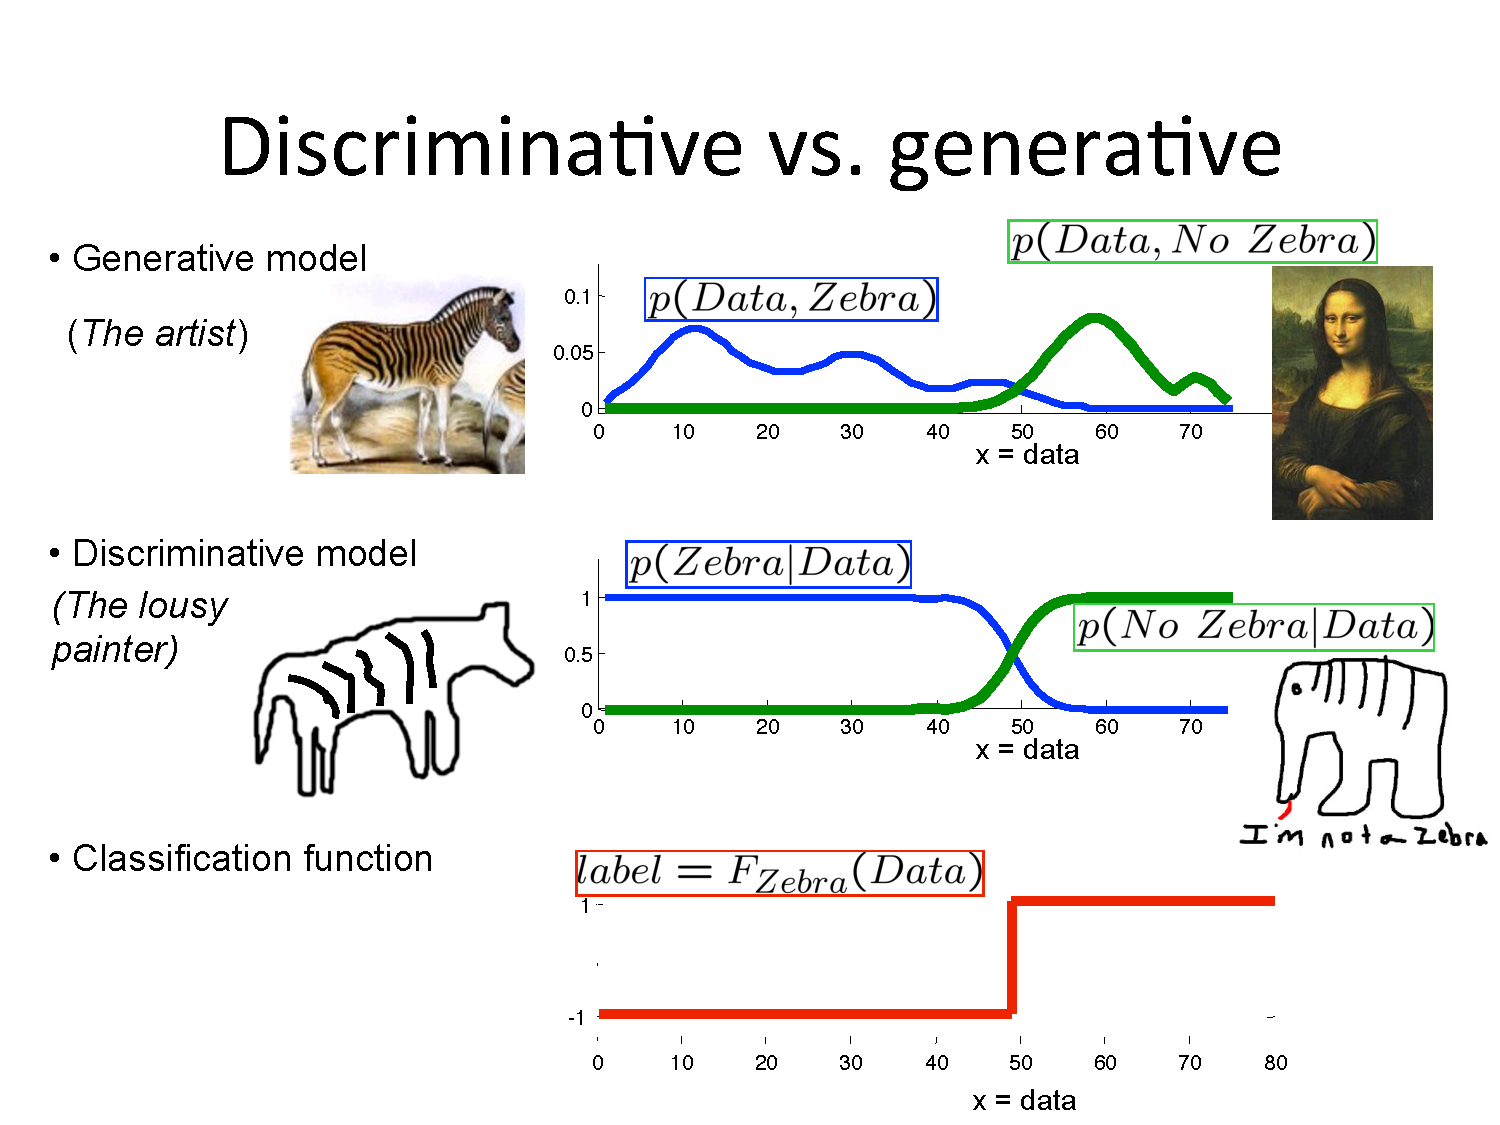
\includegraphics[width=2.5in]{figures/zebra_painting.pdf}
Why does the generative p graph max out at 0.1 and the discriminative at 1?   
    Discriminating against zebra or not zebra.  Has to sum to 1.  
    The discriminative doesn't have to sum to 1.  Many other things have to sum with it to sum to 1. 
		

